\section{Touch sensor}
\begin{figure}[H]
    \centering
    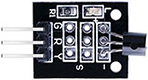
\includegraphics[angle=0, keepaspectratio=true, scale=1, width=200px, height=200px]{images/touch_sensor.jpg}
    %\caption{Caption}
\end{figure}
\subsection*{Description}
This touch sensor module detects changes in capacitances which occur when it is touched by human skin. It has both an analog and digital output but only the digital output is useful.

\subsection*{Pin mapping}
This pin mapping corresponds to the pins from left to right with the module pins facing towards you.
\begin{table}[H]
    \centering
    \begin{tabular}{|c|c|c|c|c|}
    \hline
    Index &Label &Type &Name &Description\\ \hline
    0 &A0 &Analog output &A0 &Unused\\ \hline
    1 &G &Ground &GND &\\ \hline
    2 &+ &Source voltage &$V+$ &Module source voltage ($5V$)\\ \hline
    3 &D0 &Digital output &D0 &\\ \hline
    \end{tabular}
    %\caption{Caption}
    %\label{tab:my_label}
\end{table}
\subsection*{Operation}
The output voltage at the digital pin (D0) is high when the sensor is not being touched and high when the module detects a touch. The on board LED mimics D0 and will turn on when a touch is detected. The potentiometer on the module can be used to adjust sensitivity of the sensor if the LED is on when the sensor is not being touched or if the LED does not turn when the sensor is being touched.
\subsection*{Code}
Refer to listing \ref{python_touchsensor}.
%\lstinputlisting[caption=test]{laser.py}